
\subsection{Stave Quality Assurance}
%
%
% Reviewed by Alessandro on April 9, 2015 following Allan comments on CDS (Draft version 0.6)
%
%%%%%%%%%%%%%%%%%%%%%%%%%%%%%%%%%%%%%%%%%%%%%%%%%%
A QA at the integration site for all the produced staves was performed in order to select the best staves for being integrated on the IBL support structure. The QA was also essential for ranking the staves and select the best one for being loaded around the IPT. In the following text a description of the quality assurance tests and the selection criteria for the stave integration is presented.

\subsubsection{Reception tests}
In the stave QA test~\cite{StaveQA_note} stand, loaded staves were connected to the necessary services and read-out components to be as close as possible to operation conditions in the ATLAS environment. The setup had the capability to operate two staves concurrently. 
The staves were installed in an environmental box, which was flushed with dry air to control the humidity to stay at less than \SI{3}{\percent}. The cooling system, as at the loading site, was CO$_2$ based.
%The temperature on the staves is driven by the TRACI (Transportable Refrigerator Apparatus for CO$_2$ Investigation) cooling plant which uses CO$_2$ as refrigerator as in the operation phase. The Detector Control System (DCS) and Data Acquisition (DAQ) components are connected to an End-of-Stave (EoS) PCB, which is connected to the stave in this specific setup to allow testing but it is not meant for the final detector.
Most of the DCS components were slightly modified Pixel Detector DCS components located in a rack close to the setup. The DAQ was the same as the one used in the loading site.\\
%
%\begin{figure}[!htb]
%    \centering
%    \includegraphics[width=0.9\textwidth]{Images/IBL_paper/chapter06_LoadingQA/stave_qa_schematic.pdf}
%    \caption{Schematic of the Stave QA test stand, showing the environmental box and its connections to the DCS and DAQ~\cite{StaveQA_note}.}
%    \label{fig:setup}
%\end{figure}
%%OPTICAL INSPECTION
A detailed optical inspection of each stave was performed, as first step photographs of each module were taken with high resolution camera and then a microscope investigation performed.
The full two-step optical inspection procedure was repeated after all remaining QA tests have been completed to ensure that nothing was damaged during the QA process.

Before running calibration measurements, the basic electrical functionality of a stave had to to be verified. This includes power-up studies, verification of set voltages and consumed currents in un-configured and configured states of the chip, as well as I-V characteristics of the sensors.

%Once a stave a is fully connected to the cooling and all the services, it is vital to check the sense lines of the LV power regulators are connected properly. This is done in a specific procedure where the voltage supplied to the regulators is lowered to a point, where even with a faulty sense connection the regulators cannot apply an over voltage to the chips. A correct connection of the sense lines is then easily recognisable by a voltage reading via the sense lines.

The powering behavior of the modules was tested by a LV cycle, which executed ten power cycles. In the case of faulty modules, the current consumption veried significantly between cycles. %An example for such a LV cycle is shown in Figure~\ref{fig:LVcycle} for stave ST12. Not stable currents are faced in the un-configured state when registers are improperly reset and remained in an unknown state. 
The modules passed the test provided the powering group current is below 2\,A and above 0.8\,A.

%\subsubsection{IV scans}
An I-V scan was performed for all the powering sectors. The sensor HV was ramped in 20 steps from \SI{0}{\volt} to \SI{100}{\volt} for 3D sensors and from \SI{0}{\volt} to \SI{200}{\volt} for planar sensors. The current limit for all IV measurements was \SI{20}{\micro\ampere}.
%While 3D FBK sensors show a rather steep break-down behavior well below \SI{50}{\volt}, 3D CNM sensors usually show a rather smooth break-down behavior, spread over a wide voltage range but usually below \SI{100}{\volt}, and planar sensors usually stand up to \SI{200}{\volt} (for both irradiated break-down behavior see \cite{IBL_mod_proto}).  An example for ST12 is shown in Figure~\ref{fig:IVcurves}.
%The IV curve indicates potential issues with the sensors such as unwanted surface currents or cracks.
%induced by scratches or conducting pieces bridging the guard rings.
%It is important that the required set voltage, \SI{20}{\volt} for 3D and \SI{80}{\volt} for planar sensors, can be safely applied and that the sensors show a constant leakage current over time.

%\begin{figure}
%	\centering
%		 \subfloat[\label{fig:LVcycle}]{\includegraphics[width=0.47\textwidth]{Images/IBL_paper/chapter06_LoadingQA/ST12_LVcylces.pdf}}
%		 \subfloat[\label{fig:IVcurves}]{\includegraphics[width=0.48\textwidth]{Images/IBL_paper/chapter06_LoadingQA/ST12_IVcurves.pdf}}
%	\caption[]{LV cycles (\subref{fig:LVcycle}) and sensor IV (\subref{fig:IVcurves}) characteristics for all DCS groups of ST12~\cite{StaveQA_note}.}
%	\label{fig:PoweringPlots}
%	
%\end{figure}

%After a first successful power-up of the stave, a number of values are recorded including the temperature, set voltage reading, unconfigured current and high voltage leakage current of each powering group. Expected values of these quantities are listed in Table~\ref{tab:rec_test}.
%
%\begin{table}[!htb]
%\centering
%\begin{tabular}{lcc}
%\hline\hline
%Quantity & Expected Value \\
%\hline
%Temperature & \SI{22}{\celsius} \\ %[when powered?]
%Set Voltage & \SI{2.1}{\volt}\\
%Unconfigured current & \SI{1.1}{\ampere}\\
%Configured current & \SI{1.5}{\ampere}\\
%Leakage current & \SI{<2}{\micro\ampere}\\
%\hline\hline
%\end{tabular}
%\caption{Data recorded for each powering group in the reception test and their expected values~\cite{StaveQA_note}.}
%\label{tab:rec_test}
%\end{table}
%
%A digital test is run to ensure that all modules configure and the configured current of each module group is subsequently recorded. A series of test injection commands and read out, is executed with the sensor being biased: a digital scan, a threshold scan, a ToT scan and a crosstalk scan.
%These scans give a first overview of the stave functionality and an indication of potential changes or damages \itemnduced during transport. The trend of the leakage current of each module group is closely monitored to ensure stability over time. The HV is then turned off and another threshold scan is run. Comparing the threshold scan with and without HV, areas of disconnected bumps can be identified since a pixel that is no longer connected to the sensor is not affected by the higher noise present when the sensor is not fully depleted. However, this check only gives a rough estimate and a source scan is needed to fully identify all disconnected bumps. A comparison with results from previous testing sites is made and archived together with the exact scan run numbers for future reference.
%
%
% Reviewed by Alessandro on April 9, 2015 following Allan comments on CDS (Draft version 0.6)
%
%%%%%%%%%%%%%%%%%%%%%%%%%%%


\subsubsection{Calibration and radioactive source scan}

The discriminator threshold and the Time-over-Threshold (ToT) parameters of the IBL chips needed to be calibrated and tuned to distinguish between a charged particle hit and electronic noise as well as to ensure that the charge determination was uniform over all IBL pixels. The calibration is required many times over the course of the IBL lifetime to compensate for the effects of radiation damage and for changes in operating conditions. For example, the threshold had to to be lowered as the charge collection efficiency decreases with increasing radiation damage. While the majority of the QA tests are performed at room temperature of \SI{22}{\celsius}, the staves are also cooled to the Pixel Detector operating temperature of \SI{-12}{\celsius} to test the calibration capabilities of the IBL chips in all operation environment. The module tunability was tested for reference thresholds of \SI{3000}{\e} at \SI{22}{\celsius} and \SI{1500}{\e} at \SI{-12}{\celsius}. The ToT is tuned to ~10 units of \SI{25}{\nano\second} for a reference minimum ionizing charge of \SI{16000}{\e}.

%The results of calibration to the reference thresholds of \SI{3000}{\e} at \SI{22}{\celsius} and \SI{1500}{\e} at \SI{-12}{\celsius} are listed in Table~\ref{table:calib_summary}. It should be noted that the minimal dispersion value is \SI{40}{\e} as dictated by the injection circuit. 
Figure~\ref{fig:ThresholdPerPixel} shows the threshold and noise distributions of pixels for the \SI{3000}{\e} threshold tuning at \SI{22}{\celsius} module temperature, and the \SI{1500}{\e} distribution look similar.
%%%%%%%%%%
% THIS EXPLANATION SHOULD NOT BE NECESSARY ANYMORE IF WE ONLY TALK ABOUT 14 STAVES!
The higher noise of FBK pixels was primarily due to two modules located on staves 14 and 20 at the highest $\eta$ position, the worst of which formed a small occupancy peak near \SI{300}{\e} noise. These staves were not chosen for the IBL and remain as backups in case of problems during integration. In both cases, the staves were tested on the bench of the QA setup and the HV bias supply line serving the 3D modules on the A-side is known to have \SI{0.2}{\volt} noise. In general, sensitivity to such external noise is observed for all 3D modules, more so for the FBK sensors than for the CNM sensors.
%
%\begin{table}
%\renewcommand{\arraystretch}{1.2}
%\centering
%\begin{tabular}{llccccc}
%\hline\hline
%Tuned Threshold & Pixel Type & Std. Dev. [\SI{}{\e}] & Noise [\SI{}{\e}] & Threshold over Noise\\
%\hline
%\multirow{4}{*}{3000~$e$\ at 22$^\circ$C} 	& Planar Normal	& 37.3 & $122.8\pm 9.8$ & $24.6\pm 2.0$ \\
%		                & Planar Long	& 58.1 & $146.4\pm 14.9$ & $20.7\pm 2.1$\\
%                               & 3D FBK		& 39.1 & $171.3\pm 25.0$ & $17.8\pm 2.4$\\
%                                & 3D CNM		& 40.4 & $148.9\pm 15.4$ & $20.3\pm 2.1$\\
%\multirow{4}{*}{\SI{3000}{\e} at \SI{22}{\celsius}} 	& Planar Normal	& 37 & \num{123\pm 10} & \num{25\pm 2} \\
%		                & Planar Long	& 58 & \num{146\pm 15} & \num{21\pm 2}\\
%                                & 3D FBK		& 39 & \num{171\pm 25} & \num{18\pm 2}\\
%                                & 3D CNM		& 40 & \num{149\pm 15} & \num{20\pm 2}\\
%\hline
%\multirow{4}{*}{1500~$e$\ at -12$^\circ$C} 	& Planar Normal	& 42.4 & $128.8\pm 12.9$ & $11.8\pm 1.2$\\
%                                & Planar Long	& 46.7 & $148.7\pm 16.1$ & $10.2 \pm 1.1$\\
%                                & 3D FBK		& 45.6 & $170.6\pm 24.9$ & $9.0\pm 1.2$\\
%                                & 3D CNM		& 40.8 & $146.3\pm 16.4$ & $10.4\pm 1.2$\\
%\multirow{4}{*}{\SI{1500}{\e} at \SI{-12}{\celsius}} 	& Planar Normal	& 42 & \num{129\pm 13} & \num{12\pm 1}\\
%                                & Planar Long	& 47 & \num{149\pm 16} & \num{10 \pm 1}\\
%                                & 3D FBK		& 46 & \num{171\pm 25} & \num{9\pm 1}\\
%                                & 3D CNM		& 41 & \num{146\pm 16} & \num{10\pm 1}\\
%\hline\hline
%\end{tabular}
%\caption{Threshold calibration summary for different pixel types for 18 qualified staves. Listed values are the standard deviation of the threshold, mean noise and its standard deviation, and mean threshold over noise and its standard deviation. Both tunings were performed for a 10 units of \SI{25}{\nano\second} ToT response at \SI{16000}{\e}. Long pixels of planar sensors are listed separately as they show a higher noise due to their larger pixel size. The measured threshold does not represent the in-time threshold, as no timing constraints were set. The number of pixels per type are 11,321,900;  290,304; 1,935,360 and 1,935,360 for normal planar, long planar, 3D FBK and 3D CNM pixels, respectively~\cite{StaveQA_note}.}
%\label{table:calib_summary}
%\end{table}
%
\begin{figure}
        \centering
        \subfloat[\label{fig:ThrPerPix}]{ \includegraphics[width=0.48\textwidth]{Images/IBL_paper/chapter06_LoadingQA/ThrPerPix}}
        \subfloat[\label{fig:ThrSigPerPix}]{\includegraphics[width=0.48\textwidth]{Images/IBL_paper/chapter06_LoadingQA/ThrSigPerPix}}
        \caption{Threshold (\subref{fig:ThrPerPix}) and noise (\subref{fig:ThrSigPerPix}) of pixels for \SI{3000}{\e} threshold tuning at \SI{22}{\celsius} module temperature. No constraints on timing were set for the threshold measurement.}
         \label{fig:ThresholdPerPixel}
\end{figure}


The threshold-over-noise distributions of pixels for \SI{3000}{\e} and \SI{1500}{\e} tunings are presented in Figure~\ref{fig:ThresholdOverNoise}. 
The expected physics occupancy for the IBL is \num{e-3} hits per pixel per units of \SI{25}{\nano\second} in early operation and higher in later years. 

A threshold over noise value higher than 5 ensured that the noise contamination in physics hits from IBL would be less than \SI{0.1}{\percent}. A pixel was classified as noisy when it has a noise occupancy higher than \num{e-6}, the observed fraction of noisy IBL pixels is less than \SI{0.03}{\percent} for the \SI{1500}{\e} reference tuning at \SI{-12}{\celsius} module temperature.
\begin{figure}
        \centering
        \subfloat[\label{fig:ThtOverSigPerPix}]{\includegraphics[width=0.48\textwidth]{Images/IBL_paper/chapter06_LoadingQA/ThrOverSigPerPix}}
        \subfloat[\label{fig:ThrOverSigPerPix_1500e}]{\includegraphics[width=0.48\textwidth]{Images/IBL_paper/chapter06_LoadingQA/ThrOverSigPerPix_1500e}}
        \caption{Threshold over noise distribution of pixels for \SI{3000}{\e} (\subref{fig:ThrOverSigPerPix}) and \SI{1500}{\e} (\subref{fig:ThrOverSigPerPix_1500e}) threshold tunings at \SI{22}{\celsius} and \SI{-12}{\celsius} module temperatures, respectively.}
         \label{fig:ThresholdOverNoise}
\end{figure}

%Figures~\ref{fig:thresh_mean} and~\ref{fig:thresh_sigmamean} show the threshold and threshold noise distributions, respectively, averaged over all 18 qualified staves as a function of chip number. The uncertainties displayed are twofold. The error bars represent the root mean square value to show the spread between the different staves whereas the solid squares represent the asymmetric data points with the largest deviation from the mean value. Overall, it is possible to tune all production staves down to \SI{1500}{\e} with a deviation of maximally \SI{40}{\e}. This can be seen by the flat distribution in Figure~\ref{fig:thresh_mean}. The average threshold noise value is about \SI{130}{\e} for planar sensors and still well below \SI{180}{\e} for 3D sensors. Slightly higher noise is observed on the A-side of the setup. This is due to a combination of increased noise on the HV lines of the setup and the fact that FBK modules, which are in general more sensitive to external noise, were more frequently chosen over CNM modules for loading on this side.
%
%\begin{figure}[h!]
%        \centering
%        \subfloat[\label{fig:thresh_mean}]{ \includegraphics[width=0.48\textwidth]{Images/IBL_paper/chapter06_LoadingQA/Threshold_18}}
%        \subfloat[\label{fig:thresh_sigmamean}]{\includegraphics[width=0.48\textwidth]{Images/IBL_paper/chapter06_LoadingQA/Derived_Noise_18}}
%        \caption{Average threshold (\ref{fig:thresh_mean}) and  threshold noise (\ref{fig:thresh_sigmamean}) distributions for all 18 qualified staves as a function of chip number~\cite{StaveQA_note}.}
%         \label{fig:thresh}
%\end{figure}


%%%%%%%%%%%%%%
%\subsubsection{Source Scans}%%
%%%%%%%%%%%%%%
%\begin{figure}
%        \centering
%        \subfloat[\label{fig:source_occ}]{\includegraphics[width=0.48\textwidth]{Images/IBL_paper/chapter06_LoadingQA/ST12_C5-1_source_occupancy_int}}
        %\subfloat[\label{fig:source_occall}]{\includegraphics[width=0.48\textwidth]{Images/IBL_paper/chapter06_LoadingQA/OccSr90PixelFamilies_ALL_18staves_normalized}}
%	 \subfloat[\label{fig:SourcePix}]{\includegraphics[width=0.48\textwidth]{Images/IBL_paper/chapter06_LoadingQA/source_tot_type}}
%        \caption{Typical source scan hit map of a module (\ref{fig:source_occ}) and the distribution over all chips of the most probable cluster ToT value obtained with a Landau-Gauss fit (\subref{fig:SourcePix}) ~\cite{StaveQA_note}.}
%         \label{fig:sourcescanmod}
%\end{figure}

The source scans were performed with two $^{90}$Sr sources of \SI{28.8}{\mega\becquerel} each, emitting \SI{2.28}{\mega\ev} electrons, at \SI{22}{\celsius}. The FE-I4 chip was using an internal self trigger mechanism, so that no external trigger system was required.The FE-I4s were tuned at \SI{3000}{\e} threshold and a ToT response of 10 counts in units of \SI{25}{\nano\second} at \SI{16000}{\e} signal. As the source was moved over the stave, data were taken for \SI{400}{\second} for each chip to collect reasonable statistics for identifying disconnected bumps ($\sim$200 hit per pixel).
% An example of a source scan hit map can be seen in Figure~\ref{fig:source_occ}. Regions with a lower number of hits are clearly visible and match precisely the areas where passive components are mounted on the module flex PCB. Each normal pixel has around 150 to 200 hits while long pixels in the outer columns have nearly twice as many hits, which is expected due to their size. The difference in number of hits between working and not working pixels is large enough to readily identify dead and disconnected pixels. %Figure~\ref{fig:source_occall} shows the occupancy distribution for the three different sensor flavours. The mean occupancy for planar sensors is slightly lower than for 3D sensors because they have a thickness of \SI{200}{\micro\meter} compared to \SI{230}{\micro\meter} in the 3D case and thus have a shorter interaction length. The occupancy for CNM sensors, however, is slightly lower than for FBK since in that design the electrodes are not as deeply etched as for FBK sensors and thus leave some less active regions close to surface.

%Although source scans are mainly used to identify disconnected bumps, it is also possible to check the charge calibration of each chip as the $^{90}$Sr emits mips. If only clusters with more than one hit are used, the ToT distribution is slightly shifted to higher values, however it is still possible to compare the relative charge calibration of all chips. %Figure~\ref{fig:SourceClus} shows the average most probable value of the Landau-Gauss fit and its dispersion as a function of position on a stave. 
%The one dimensional distribution of the most probable value of each chip is plotted in Figure~\ref{fig:SourcePix}. There is no dependance on the position on the stave and the mean most probable ToT value is \num{9.9\pm 0.4} in units of \SI{25}{\nano\second}.
%
%\begin{figure}[h!]
%        \centering
%        \subfloat[\label{fig:SourceClus}]{\includegraphics[width=0.48\textwidth]{Images/IBL_paper/chapter06_LoadingQA/source_tot_dist}}
%        \subfloat[\label{fig:SourcePix}]{\includegraphics[width=0.48\textwidth]{Images/IBL_paper/chapter06_LoadingQA/source_tot_type}}
%        \caption{Most probable cluster ToT value obtained from a Landau-Gauss fit, (\subref{fig:SourceClus}) shows the average as a function of chip number and (\subref{fig:SourcePix}) shows the distribution over all chips~\cite{StaveQA_note}.}
%         \label{fig:SourceToT}
%\end{figure}

%%%%%%%%%%%%%
\subsubsection{Pixel defects}%%
%%%%%%%%%%%%%
Pixel defects can be categorized into three main ``bad pixel" classes: defects pertaining to the front-end, sensor or bump bonding. A combined analysis of the calibration and source scan results makes it possible to classify each failing pixel. The failure classification is exclusive, which means that only one category of failure is used per pixel. All failure categories are listed in order of exclusion in Table~\ref{tab:badpix}, showing the category name, scan used for identification and the specific criteria for each class.
%
\begin{table}
    \centering
    \begin{tabular}{lccc}
    \hline\hline
        Failure Name & Scan Type & Criteria & \\
        \hline
        Digital Dead & Digital Scan & Occupancy \SI{<1}{\percent} of injections \\
        Digital Bad & Digital Scan & Occupancy \SI{<98}{\percent} or \SI{>102}{\percent} of injections \\
        Merged Bump & Analog Scan & Occupancy \SI{<98}{\percent} or \SI{>102}{\percent} of injections\\
        & Crosstalk Scan & Occupancy \SI{>80}{\percent} of \SI{25}{\kilo\ev} injections  \\
        Analog Dead & Analog Scan & Occupancy \SI{<1}{\percent} of injections  \\
        Analog Bad & Analog Scan & Occupancy \SI{<98}{\percent} or \SI{>102}{\percent} of injections \\
        Tuning Failed & Threshold Scan & s-curve fit failed   \\ %(threshold = 0~$e$)
         & ToT Test & ToT response is 0 or 14 $\times$ \SI{25}{\nano\second}& \\
        Noisy & Noise Scan & Occupancy \num{>e-6} hits per \SI{25}{\nano\second} &\\
        Disconnected Bump & Source Scan ($^{90}$Sr) & Occupancy \SI{<1}{\percent} of mean Occupancy & \\
        High Crosstalk & Crosstalk Scan & Occupancy \num{>0} with \SI{25}{\kilo\e} injection & \\
        \hline\hline
    \end{tabular}
    \caption{Classification of pixel failures\label{tab:badpix}.}
\end{table}
%
\begin{figure}
        \centering
%        \subfloat[\label{fig:disc3D}]{\includegraphics[width=0.48\textwidth]{Images/IBL_paper/chapter06_LoadingQA/disc3D_18}}
%        \subfloat[\label{fig:discplanar}]{\includegraphics[width=0.48\textwidth]{Images/IBL_paper/chapter06_LoadingQA/discplanarLR_18}}
%				\\
%        \subfloat[\label{fig:badnodisc}]{\includegraphics[width=0.48\textwidth]{Images/IBL_paper/chapter06_LoadingQA/badnodisc_18}}
        \subfloat[\label{fig:bad_per_stave}]{\includegraphics[width=0.48\textwidth]{Images/IBL_paper/chapter06_LoadingQA/badpix_per_stave}}
        \subfloat[\label{fig:BadPixelCorrelation}]{\includegraphics[width=0.48\textwidth]{Images/IBL_paper/chapter06_LoadingQA/BadPixelCorrelation}}
       \caption{ \subref{fig:bad_per_stave}Total number of bad pixels per stave for all 18 qualified staves. 	\subref{fig:BadPixelCorrelation} Number of bad pixels per chip after module assembly at the module
production site and after stave loading in the stave QA. In general the
number of bad pixels is lower in the stave QA, which can be related to a
more strict set of scans performed in the module production. A very small
amount of chips have a higher amount of bad pixels in the stave QA which
can be accounted for by differences in the calibration}
       
         \label{fig:baddiscfull}
\end{figure}

Most of the failures rely on the module showing a hit excess or deficit. The digital and analog functionality can be directly tested with digital and analog scans, respectively. Digital and analog dead pixels are common electronic failures, while the digital and analog bad categories only appear in high numbers in case of a low ohmic connection between pixels. The latter mainly occurred in the early prototype production of modules and is now fixed. An exception to a failing analog functionality is the identification of a merged bump. It is defined as two solder bumps connecting the sensor to the read-out chip being merged together and manifests itself in an analog failing pixel which still gives a response in an crosstalk scan. A pixel is classified as untunable if the threshold or ToT cannot be tuned at all, however a high discrepancy from the tuning target is allowed as these kinds of pixels can still be used for operation even if just to a limited extent. The noise occupancy, which shows how many hits per BC are produced due to noise, is a very important quantity for operation. A pixel gets masked for operation and classified as a bad pixel if the noise occupancy exceeds \num{e-6} hits per units of \SI{25}{\nano\second}. All tests mentioned so far are aimed at probing the electrical functionality of the pixel. In addition, it is necessary to ensure that the read-out electronics are properly connected to the sensor, in other words to make sure that the bump connection in-between is intact. The easiest way to identify a disconnected bump, is to analyze the response from a source scan. If a pixel shows zero or only very few hits in the source scan data, the bump is assumed to be disconnected. The last bad pixel category, called high crosstalk, is not directly related to the performance of the pixel but if a sensor pixel shows a high amount of charge sharing to its neighbours this can influence the precision of the offline reconstruction.

%The total number of bad pixels over all chips for geographical pixel position can be seen in percentage in Figure~\ref{fig:baddiscfull}. No clear correlation between the chip topology, other than edge regions, and the measured disconnected bumps are found. There is a clear increase in the number of bad pixels as one moves to higher $\eta$ values. This behaviour is explained by the strategy chosen to load the best modules into the central region of a stave. %The exact numbers per bad pixel category are collected for each stave in Table~\ref{table:badpixsummary}.
%
%\begin{table}[!htbp]
%\renewcommand{\arraystretch}{1.0}
%\centering
%\begin{tabular}{lccccccccc}
%\hline \hline
%Stave & Digital & Analog & Disconnected & Merged & Untuneable & Noisy & Crosstalk & Total \\
%\hline
%ST01 & 6 & 389 & 272 & 3 & 232 & 11 & 98 & 1011 \\
%ST02 & 10 & 255 & 54 & 3 & 117 & 15 & 125 & 579 \\
%ST03 & 6 & 375 & 473 & 0 & 182 & 21 & 178 & 1235 \\
%ST04 & 2 & 201 & 254 & 0 & 275 & 8 & 59 & 799 \\
%ST05 & 2 & 207 & 172 & 0 & 183 & 4 & 33 & 601 \\
%ST06 & 6 & 206 & 337 & 0 & 147 & 9 & 29 & 734 \\
%ST09 & 8 & 360 & 476 & 3 & 167 & 8 & 88 & 1110 \\
%ST10 & 16 & 179 & 304 & 0 & 141 & 3 & 3 & 646 \\
%ST11 & 10 & 196 & 159 & 0 & 155 & 8 & 37 & 565 \\
%ST12 & 15 & 172 & 169 & 0 & 166 & 7 & 13 & 542 \\
%ST13 & 9 & 127 & 205 & 0 & 336 & 6 & 35 & 718 \\
%ST14 & 4 & 161 & 1364 & 0 & 330 & 7 & 11 & 1877 \\
%ST15 & 5 & 222 & 350 & 0 & 259 & 20 & 8 & 864 \\
%ST16 & 1 & 237 & 414 & 1 & 187 & 15 & 24 & 879 \\
%ST17 & 2 & 214 & 598 & 0 & 229 & 5 & 4 & 1052 \\
%ST18 & 13 & 161 & 902 & 1 & 178 & 2 & 9 & 1266 \\
%ST19 & 10 & 163 & 543 & 0 & 228 & 11 & 16 & 971 \\
%ST20 & 14 & 224 & 1051 & 0 & 535 & 13 & 302 & 2139 \\
%\hline \hline
%\end{tabular}
%\caption{Overview of the number of different bad pixel categories for the 18 qualified staves~\cite{StaveQA_note}.}
%\label{table:badpixsummary}
%\end{table}
%A production cut of 100 bad pixels per chip is applied after assembly of the modules. Some of the modules on the IBL staves are above this cut, because the cut was relaxed to the end of the production when there was a shortage of 3D sensor assemblies. \SI{73}{\percent} of all chips loaded onto staves have less then \SI{0.1}{\percent} bad pixels.

The total number of failing pixels per stave is shown in Figure~\ref{fig:bad_per_stave}. The two dashed lines indicate \SI{0.1}{\percent} and \SI{0.2}{\percent} marks, the specification requires a stave to be below \SI{1}{\percent}. All staves are well below this cut, \SI{80}{\percent} of staves are below the \SI{0.2}{\percent} mark and \SI{50}{\percent} of those staves are even below \SI{0.1}{\percent}. About \SI{50}{\percent} of all failures are due to disconnected bumps, the other \SI{50}{\percent} are distributed between a pixel being analog dead or its tuning being impossible.\\
Figure \ref{fig:BadPixCorrelation} presents the correlation of the number of bad pixels per FE detected in the module production and stave QA. A correlation can be observed. Although similar cuts to classify a pixel as bad have been used in the two test stages, during the module production the more intense test procedure was applied. This explains why more bad pixels are detected per FE in the module production.


%
%\begin{figure}[h!]
%        \centering
%        \subfloat[\label{fig:BadPixelCorrMapDC}]{\includegraphics[width=0.48\textwidth]{Images/IBL_paper/chapter06_LoadingQA/BadPixelComparrisonMapDC}}
%        \subfloat[\label{fig:BadPixelCorrMapSC}]{\includegraphics[width=0.48\textwidth]{Images/IBL_paper/chapter06_LoadingQA/BadPixelComparrisonMapSC}}
%        \caption{Bad pixel correlation map for DC (a) and SC (b) modules for the detection of geographical areas with increased number of bad pixels after stave loading. For each pixel tagged as bad in the stave QA but not in the module production, the bad pixel difference is increased by one, while it is decreased by one for the opposite scenario~\cite{StaveQA_note}.}
%         \label{fig:BadPixCorrMap}
%\end{figure}
%A significant increase of bad pixels in geographical areas, for example the chip edges, would be a sign of damage evoked by module transport, handling or loading to the stave. To identify such areas an overlay map of all modules loaded on staves is used, see figure \ref{fig:BadPixCorrMap}. The entry for each pixel position is increased by one if the pixel was detected as bad in the stave QA, but not in the module QA. In the opposite scenario the entry is decreased by one. If a pixel is detected bad in both or none of the test stages, the entry is not changed. With this procedure the randomly distributed pixels which were not working due to the calibration either at the module production site or the stave QA should fluctuate around zero. Again the more strict test procedure in the module production results in a slight negative offset in this representation. No prominent areas can be observed, the clusters of new bad pixels in the corner regions of the chip which would point to disconnection of the bumps are not statistical significant enough to show a systematic effect. 

\subsubsection{Stave ranking}
%
%   Reviewed by Alessandro on April 9, 2015 following Allan comments on CDS (Draft version 0.6)
%
%%%%%%%%%%%%%%%%%%%%%%%%%%%%%%%%%%


Among the 18 qualified loaded staves, it is not trivial nor unique how to select and map 14 staves to integrate as the parts of the IBL. We chose the geometrical acceptance loss due to bad pixels as the main concern to select staves.

The quality of a loaded stave with respect to geometrical acceptance inefficiency due to bad pixels can be scored with $\eta$-weighted bad pixel fraction $V$ defined as
\begin{eqnarray}
    V = \frac{\sum_{i~\in~{\rm bad~pixels}}\cosh^{-1}(\eta_{i})}{\sum_{i~\in~{\rm all~pixels}}\cosh^{-1}(\eta_{i})}
\end{eqnarray}
where the factor $\cosh(\eta_{i})^{-1}$ is the weight of the geometrical acceptance of the pixel $i$ measured in the $\eta$-$\phi$ coordinate system.

Not only the total dead area, but also localisation of the dead area is considered to be disfavoured. A permutation algorithm was developed to select which stave select for a given position\cite{StaveQAnote}.

%In order to seek a good permutation, we developed a selection algorithm described as follows. For the given permutation of the staves labeled as $k$, we can calculate the two-point correlation function of the bad pixels defined as
%\begin{eqnarray}
%C_{k}(\varDelta r) &\equiv& \sum_{i,j\in {\rm bad\,pixels}}\frac{1}{\cosh(\eta_{i})}\frac{1}{\cosh(\eta_{j})}\delta(\varDelta r_{ij}-\varDelta r),\\
%\varDelta r_{ij} &=& \sqrt{ (\eta_{i}-\eta_{j})^{2} + (\phi_{i}-\phi_{j})^{2}}
%\end{eqnarray}
%where ($\eta_{i},\phi_{i}$) is the coordinate of the pixel $i$. Before calculating $C_{k}(\varDelta r)$, the bad pixel distribution was convoluted with gaussian in $z$-axis with $\sigma_{z} = 2.5~{\rm cm}$ corresponding to the fluctuation of the beam size. $C_{k}(\varDelta r)$ can be compared with the uniform bad pixel distribution $C_{\rm uni}(\varDelta r)$, where the relative scale of $C_{k}(\varDelta r)$ to $C_{\rm uni}(\varDelta r)$ was adjusted empirically by minimising the deviation of the two distribution at $1.0<\varDelta r<4.5$ with normalisation of $\int\!d\varDelta r\,C_{\rm uni}(\varDelta r)=1$. We define the non-uniformity of the bad pixel $D_{k}$ as
%\begin{eqnarray}
%D_{k} = \int\!d\varDelta r \left[w(\varDelta r) \left|C_{k}(\varDelta r)-C_{\rm uni}(\varDelta r)\right|^{2}\right]
%\end{eqnarray}
%where $w(\varDelta r)$ is a window function. Note that this algorithm naturally disfavours staves with large number of bad pixels, since having many bad pixels tends to make concentrate the bad pixels to specific $\phi$ region. With such measure we can compare the distribution of the bad between different choice of permutation.

%However the total number of permutations to choose 14 out of 18 qualified staves is ${\rm {}_{18}P_{14}/14}\simeq 1.9\times10^{13}$, and practically it was difficult to try every permutation to evaluate $D_{k}$. Alternately the evaluation of the non-uniformity was performed for partial permutation $k'(n)$, where only the permutation of the first $n$-slots are defined and the remaining slots are undefined\footnote{The stave integration was performed from position \#14 to \#1 sequentially.}. In this case the undefined slots are filled with pseudo-data of bad pixel distribution, where the number and the distribution of bad pixels of an undefined chip are randomly taken from those of the qualified staves. The evaluation of non-uniformity $D_{k'(n)}$ for $k'(n)$ is no longer deterministic, and we evaluate it with the median ${\tilde D}_{k'(n)}$ with repeating the random generation of the pseudo-data many times. Practically we determined $n$-th stave to integrate with fixing the permutation of the previous $(n-1)$ staves. This changeover from the ``brute force'' algorithm to ``gradual determination'' algorithm made it possible to calculate the arrangement in realistic timescale.

Two constraints were applied:
\begin{itemize}
\item the first and the last integrating staves have to have the best planarity
\item the reworked and non-reworked staves for corroded wire bonds at the DSF are mapped alternately.
\end{itemize}

Table~\ref{table:rankingsummary} summaries the position in the IBL loading map, the rank and other characteristics of the staves considered in the selection. Figure~\ref{fig:badpix_dist_eta} compares the average bad pixel ratio distribution as a function of pseudo-rapidity $\eta$ for the 14 installed staves to the four not installed staves, the former achieving better performance in terms of acceptance. The total bad pixel ratio of the integrated IBL staves is \SI{0.07}{\percent} for $|\eta|<2.5$ and \SI{0.09}{\percent} when considering the full $\eta$ range. For comparison, the corresponding numbers for the four not installed staves are \SI{0.16}{\percent} and \SI{0.18}{\percent}, respectively. Figure~\ref{fig:badratio_load_unload} shows the two-dimensional distribution of bad pixel ratios as a function of $\eta$ and $\phi$. Stave overlap is taken into account in this plot and the ratio is computed as the number of bad pixels per total number of pixels in a unit cell.

\begin{table}
\renewcommand{\arraystretch}{1.4}
\centering
\begin{tabular}{lcccccc}
\hline \hline
Position & Stave & Number of bad pixels & Score & Planarity [\SI{}{\micro\meter}] & Reworked \\
\hline
01 & ST17  & 1052 & 1.01 & 114 & no \\
02 & ST02 & 579 & 0.44 & 205 & yes \\
03 & ST19  & 971 & 1.13 & 266 & no\\
04 & ST09   & 1110 & 1.00 & 229 & yes \\
05 & ST18   & 1266 & 0.94 & 336 & no\\
06 & ST04   & 799 & 0.69 & 235 & yes \\
07 & ST13   & 718 & 0.56 & 224 & no\\
08 & ST10   & 646 & 0.62 & 243 & yes \\
09 & ST11   & 565 & 0.58 & 298 & no \\
10 & ST12   & 542 & 0.62 & 314 & yes \\
11 & ST16   & 879 & 0.82 & 329 & no \\
12 & ST06   & 734 & 0.79 & 290 & yes \\
13 & ST15   & 864 & 0.84 & 325 & no \\
14 & ST05   & 601 & 0.68 & 189& yes\\ \hline
n/a & ST01 & 1011 & 1.04 & 224 & yes\\
n/a & ST03 & 1235 & 2.48 & 223 & yes\\
n/a & ST14 & 1877 & 1.11 & 218 & no\\
n/a & ST20 & 2139 & 2.01 & 237 & no\\
\hline \hline
\end{tabular}
\caption{Ranking and loading order overview of the 14 IBL staves. The position is sequential around the beam-pipe. The cooling pipe of the stave in position 01 is at $\phi = \SI{-6.1}{\degree}$, subsequent staves are displaced by \SI{25.7}{\degree} in $\phi$. The score is determined by the number of bad pixels, each of which is weighted according to the position on a stave. A lower score thus translates into a higher quality stave. The planarity shows the difference between the minimum and maximum height of a stave. The last column indicates whether a stave has been reworked at the CERN DSF bond lab. For completeness, the bottom four lines show numbers for the staves that were not chosen for installation. For the stave loading around the beam-pipe, not only this score but a uniform $\eta-\phi$ bad pixel distribution and engineering constraints are also taken into account.}
\label{table:rankingsummary}
\end{table}



%
\begin{figure}
        \centering
       	\subfloat[\label{fig:badpix_dist_eta}]{\includegraphics[width=0.48\textwidth]{Images/IBL_paper/chapter06_LoadingQA/badpix_dist_eta_load_unload.pdf}}
        \subfloat[\label{fig:badpix_etaphi}]{\includegraphics[width=0.48\textwidth]{Images/IBL_paper/chapter06_LoadingQA/badpix_etaphi_etaphi.pdf}}
   \caption{Average bad pixel ratio distribution (\ref{fig:badpix_dist_eta}) as a function of $\eta$ for installed and not installed production staves and (\ref{fig:badpix_etaphi}) in the $\eta-\phi$ plane for the 14 IBL staves.}
    \label{fig:badratio_load_unload}
\end{figure}

\subsubsection{Wire bond corrosion issue}
In the middle of the IBL production an environmental incident occurred with the Quality Assurance set-up for which two production staves were in tests got damaged. While the staves were in operation with power and cooling at \SI{-20}{\celsius} it was discovered some electrical dysfunctions due to ice building-up around the coldest part of the staves. Further investigations revealed some defects and leaks of the environmental box which was later upgraded and much improved in term of safety.
The two staves were carefully inspected under a microscope and it was discovered that most of the aluminium wire bonds got corroded (see Figure\,\ref{fig:wire-corrosion_50}) where few were even eaten-up. The white residue or powder seen around the bond foot could be barely seen with normal incident light while with ring or raising lights this could be easily seen.
The other produced staves were carefully inspected with the same type of illumination under the microscope for which a similar observation was made.
 \begin{figure}
        \centering
        %\subfloat[\label{fig:wire-corrosion_25}]{\includegraphics[width=0.48\textwidth]{Images/IBL_paper/chapter06_LoadingQA/wire-corrosion_25.png}}
        \subfloat[\label{fig:wire-corrosion_50}]{\includegraphics[width=0.48\textwidth]{Images/IBL_paper/chapter06_LoadingQA/wire-corrosion_50.png}}
        \subfloat[\label{fig:TCplot}]{ \includegraphics[width=0.48\textwidth]{Images/IBL_paper/chapter06_LoadingQA/TCplot.pdf}}
        \caption{(a) Scanning Electron Microscopy (SEM) image of corroded wires and residues. (b) Temperature and dew point monitoring in the stave modules vicinity during the thermal cycling in the \SI{1.6}{\meter\cubed} climate chamber.}
        \label{fig:wire-corrosion}
\end{figure}
The decision was to stop the production until the origin of the problem was understood and actions taken to cure and rework the 11 out of 12 already produced staves that were affected.
%Given this major crisis a number of actions were taken as:
%\begin{itemize}
%\item Identification of the origin of the problem and in order to improve the QA system and to release the rest of the production safely
%\item Setting up a task force to investigate the corrosion issue, evaluate possible evolution of this phenomenon and identify the possible improvement like cleaning and coating.
%\item Organise a rework centre to clean all the wires and re-bond the defective stave
%\item Release an additional module production with remaining components to secure the number of IBL stave for the integration
%\end{itemize}
%The investigation started with water which is one of the essential ingredients to trigger the corrosion process. When there is a temperature excursion and when the environmental condition is not correctly controlled the risk to reach the dew point is considered to be high. Therefore and after investigation of all the QC and QA steps two set-up were identified with high risks. 

The powder was originated from the presence of water on the wire-bonds pad of the flexes, originated during the thermal cycle at the loading site and for two of the stave by an accident during the stave QA procedure.
%The first one is the climate chamber (with a volume of \SI{1.6}{\meter\cubed}) that was used to qualified the stave in a temperature range from  \SI{-40}{\celsius} to \SI{+40}{\celsius} by cycling ten times. 
Given the large volume and the fast ramp it was observed by doing a monitoring study in the vicinity of the stave modules, that the dew point was reached for a couple of minutes during the fast temperature ramp-up (see Figure\,\ref{fig:TCplot}). Even if the volume was flushed with dry air during the cycles and the humidity controlled activated, this was not enough to guaranty the absence of water. Apart from the corrosion issue the stave electrical and mechanical integrity was not affected which was confirmed with electrical characterizations and metrology surveys. For the rest of the production the newly loaded staves were not thermal cycles.
The other produced staves were carefully inspected with the same type of illumination under the microscope for which a similar, but much less severe, observation was made.
The setup used for the stave quality assurance was reviewed and qualified with prototype staves before releasing it for testing the reworked and the newly produced staves.\\
%The interconnection of the Al wire on a different metallic surface remains an issue even when at room temperature.
The interconnections between the FE and the module flex or on the module flex itself have to be made with Ni/Au pad of up to \SI{3}{\micro\meter} and \SI{100}{\nano\meter} respectively, while the wire-bonds are made of Al. Au and Al form a galvanic coupling and electro-chemistry that cause ions from the anode (aluminium is the most electro-negative) to migrate to the electrolyte to plate the cathode. During the ultrasonic wire bonding the friction generates elevated temperatures which remove locally the thin gold layer and the final metal contact is made between aluminium and nickel which is more stable with a lower galvanic coupling. In addition the aluminium wire is normally protected by a thin oxidation layer that is quickly formed after hours to stabilize at a thickness of about 5\,nm. However this layer can be damaged in presence of water or due to mechanical or chemical attack. In water and if not ultra-pure typical ionic compounds dissolved easily in water and can chemically attack the anode which is here the aluminium in the electrolyte with gold at the periphery of the bond foot.
 \begin{figure}
        \centering
        \subfloat[\label{fig:wire-corrosion_25}]{\includegraphics[width=0.48\textwidth]{Images/IBL_paper/chapter06_LoadingQA/EDSpict_1.png}}
        \subfloat[\label{fig:wire-corrosion_25}]{\includegraphics[width=0.48\textwidth]{Images/IBL_paper/chapter06_LoadingQA/EDSpict_2.png}}
        \caption{Images of a corroded Al-wire (a) and residue (b) taken from one of the accidental stave. Image was taken with an EDS analysis set-up.}
        \label{fig:wire-corrosion_EDS}
\end{figure}
The corrosion residues and Al-wires were analyzed (see Figure\,\ref{fig:wire-corrosion_EDS}) with an Energy Dispersive X-Ray Spectroscopy (EDS) technique which revealed a number atoms C, O, Ca, Na, Cl, F at a level of up to few \% which alone or in a molecular form can be the necessary ionic compounds to chemically attack the aluminium.
The presence of ionic compounds suggested improving the cleaning of the module flex after SMD assembly. The corrosion process could be reproduced easily in the laboratory in presence of deionized water on wire bonded samples. However, further investigations revealed that this process can even be observed on ultra-clean bare flex assembly.  Additional cleaning process like plasma cleaning did not even help to stop the observation of the corrosion phenomenon. The susceptibility to corrosion in term of observation of the number of bubbles while the bond feet were in immersion could depend upon the cleaning and upon the origin of the flex but never disappeared.
%An ultimate sample analysis was done with an X-ray Photoelectron Spectroscopy (XPS) and alternating the measurements and the sputtering of the gold layer with argon-ion. This method allows removing a defined and calibrated gold layer with depends upon the exposition time (\SI{0.6}{\nano\meter\per \minute}). This allows measuring the atomic spectrum at the gold surface removing layers by step until reaching the Ni interface. This measurement was made for several flex circuits and for two different producers. On one sample Fluorine was detected at a significant level (up to \SI{14}{\percent} at \SI{7}{\nano\meter}) and which could not be understood and reproduced from other flex circuits from the same producer.

\subsection{Summary of the IBL construction}
\begin{figure}
\centering
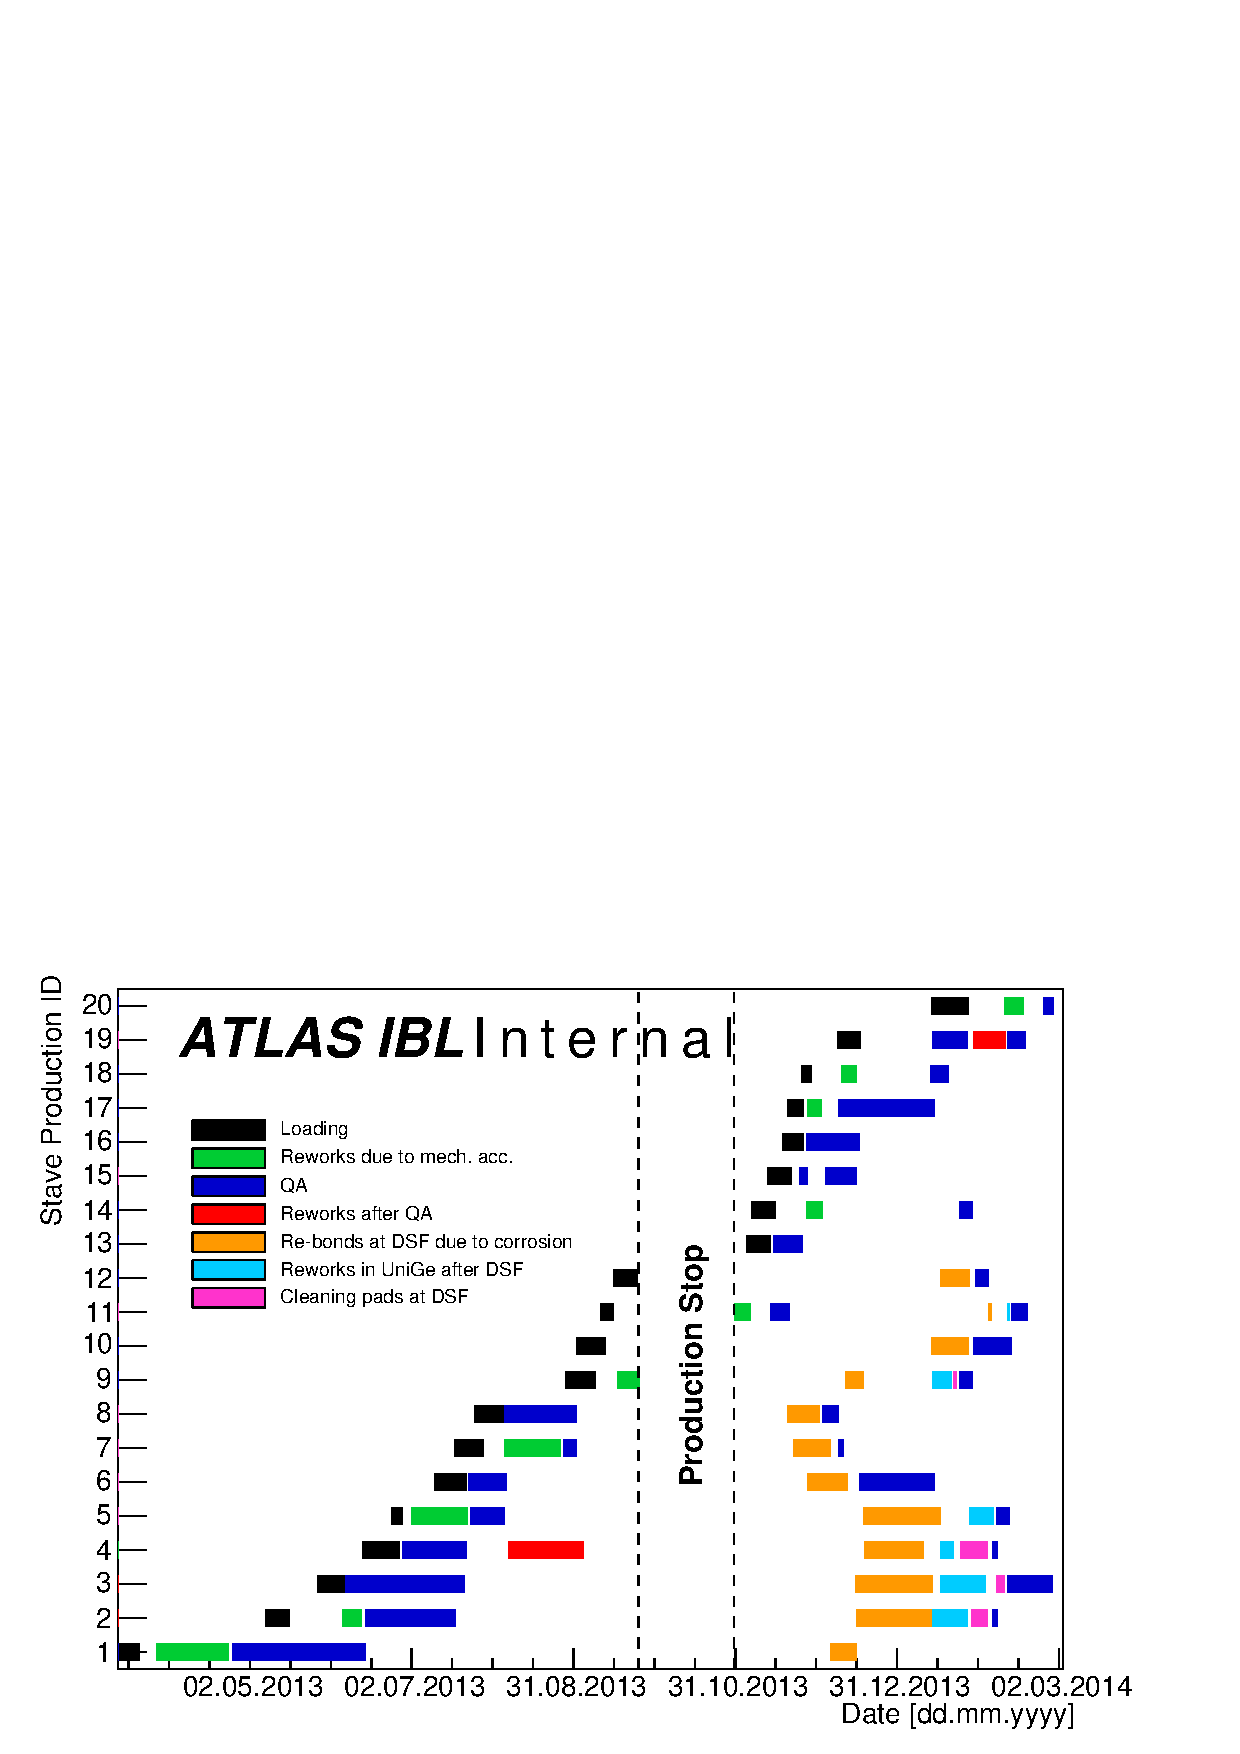
\includegraphics[width=0.8\textwidth]{Images/ibl_stave_loading/Conclusions/workFlow.pdf}
\caption{Work flow of the stave loading activity}
\label{pic:workflow}
\end{figure}
The construction of the IBL last three years and it consists of assembly steps that involved several institutes of the ATLAS collaboration. A production of xxxx FE-I4 module was done, 400 of them was loaded onto staves.
A total of 20 staves was fully produced and qualified, 18 of them was selected as a candidate for the loading and 14 of them were successfully inserted in the ATLAS volume.
The loading phase lasted one year, as shown in Figure~\ref{pic:workflow}, in which two stops happened for the investigation of the bump-bonding failure and the wire bond corrosion. Both the issue were solve and at the end of the production a detector with only 0.2$\percent$ failing pixels was inserted in the ATLAS core.
\pagebreak